\documentclass{standalone}
\usepackage{tikz}
\begin{document}
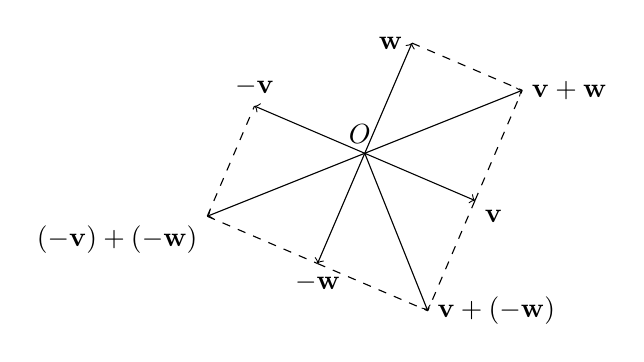
\begin{tikzpicture}[scale = 2]
    \coordinate(O)at(0,0);
    \node[above left]at(0.1,0){$O$};
    \draw[->](O)--(0.7,-0.3)node[below right]{$\mathbf{v}$};
    \draw[->](O)--(-0.7,0.3)node[above]{$-\mathbf{v}$};
    \draw[->](O)--(0.3,0.7)node[left]{$\mathbf{w}$};
    \draw[->](O)--(-0.3,-0.7)node[below]{$-\mathbf{w}$};
    \draw[->](O)--(0.4,-1)node[right]{$\mathbf{v}+(-\mathbf{w})$};
    \draw[->](O)--(-1,-0.4)node[below left]{$(-\mathbf{v})+(-\mathbf{w})$};
    \draw[->](O)--(1,0.4)node[right]{$\mathbf{v}+\mathbf{w}$};

    \draw[dashed](-1,-0.4)--(-0.3,-0.7);
    \draw[dashed](-1,-0.4)--(-0.7,0.3);
    \draw[dashed](-0.3,-0.7)--(0.4,-1);
    \draw[dashed](0.7,-0.3)--(0.4,-1);
    \draw[dashed](0.7,-0.3)--(1,0.4);    
    \draw[dashed](0.3,0.7)--(1,0.4);
\end{tikzpicture}
\end{document}